\chapter{Intrabundle - An OSGi Bundle Introspection Tool}


\section{Introduction}
It was clear in previous chapters that modular and non modular applications have many differences and specific features hence the need for dedicated approach for quality analysis. This chapter presents a tool called \emph{Intrabundle} \citep{intrabundle github 2014}, an open source Java based application created in the context of this work. Intrabundle introspects OSGi projects collecting useful information and calculates OSGi bundle and project \textbf{internal quality}.  


\section{Design Decisions}
To analyze and extract data from large code bases of OSGi projects, which can vary from KLOCs to thousands of KLOCs, there was the need of a lightweight approach. Some \emph{functional requirements} were:

\begin{itemize}
\item Analyze different formats of OSGi projects like Maven\footnote{\href{http://maven.apache.org/index.html}{Maven} is a build tool for Java}, Eclipse projects and BND\footnote{\href{http://bndtools.org/}{BND} is a tool to easy OSGi projects development}; 
\item It should be able to dive deep into projects source code like counting methods calls, differentiate classes and interfaces and so on;  
\item Get general informations like project version, revision or latest commit in source repository;
\item Should be easy analyze lots of projects;
\item Should output a detailed Human readable quality report so the extracted information can be analyzed.
\end{itemize}

and the following \emph{non functional requirements}:

\begin{itemize}
\item Only open sourced projects\footnote{Projects that have its source code made available with a license in which the copyright holder provides the rights to study, change and distribute the software to anyone and for any purpose} because we focus on internal quality where the code is important;
\item The tool should be lightweight to analyze real, complex and huge OSGi projects;
\item Find and Introspect manifest files where valuable OSGi information rely; 
\item Should be testable;
\item Fast;
\item Use Java to leverage the author's experience in the language;
\item Use a good file system API\footnote{An API expresses a software component in terms of its operations, inputs, outputs, and underlying types.} because file manipulation is one of the most frequent tasks the tool should perform.\\*
\end{itemize}
 

The following alternatives were evaluated:

\begin{enumerate}
\item Build a standalone Java client application using javaFX\footnote{\href{http://docs.oracle.com/javase/8/javase-clienttechnologies.htm}{JavaFX} is a set of graphics and media packages that enables developers to design, create, test, debug, and deploy rich client applications};
\item Create an eclipse plugin\footnote{\href{https://wiki.eclipse.org/FAQ_What_is_a_plug-in\%3F}{Eclipse plug-ins} are software components with the objective to extend Eclipse IDE};
\item Create a  Maven plugin\footnote{Maven is a build tool that consists of a core engine which provides basic project-processing capabilities and build-process management, and a host of \emph{plugins} which are used to execute the actual build tasks.};
\item Build the tool on top of JBoss Forge;
\item Extend an existing static/internal analysis tool like PMD.
\end{enumerate}

The chosen among the above options was JBoss Forge, due to the following facts:

\begin{itemize}
\item Works inside and outside eclipse;
\item Works regardless of build tool;
\item As its a command line tool its very lightweight and can analyze multiple OSGi projects at the same time;
\item The programing model is based on top of the so called CDI\footnote{Context and Dependency Injection for the Java platform. CDI is a dependency injection framework where instead of dependencies construct themselves they are injected by some external means, in cae CDI} so managing Objects lifecycle and event is handled by CDI automatically;
\item Forge has a very well established and documented file system manipulation api based on java.io;
\item Forge is very flexible so generating quality reports is a matter of using a report API inside it;  
\item The author already had experience with JBoss Forge and CDI. 
\end{itemize}

Creating an eclipse plugin for analyzing OSGi projects could be not as lightweight as forge plugin. We would need eclipse started and OSGi projects imported inside IDE so the eclipse plugin could identify the project resources.

JavaFX would require use standard Java file system manipulation api(java.io) which has many caveats and pitfalls so for example its easy to create a memory leak or too many files opens error. Also with JavaFX there the need to implement the interface/GUI which is already well done in Eclipse or Forge.

Maven plugins are limited to maven projects.

PMD\footnote{A very nice tool for static code analysis. It is based on rules that can be created via xml or xpath expression. When a rule is violated it can output warns or errors to the console} has a very limited API so it could be hard to generate reports or analyze multiple projects using it. 


\section{Implementation Overview}

Intrabundle is composed by 3 Forge plugins, see section \ref{sec:forge:plugin} for details about Forge plugins. The first is \emph{BundlePlugin} which extracts OSGi bundle information, second is \emph{OSGiPlugin} that has a vision of all bundles composed by the project. Third is OSGiScan a plugin responsible for scanning OSGi bundles recursively in file system. Another component in the architecture is \emph{MetricsCalculator} that calculates bundle and OSGi project quality based on metrics produced by OSGiPlugin and BundlePlugin.

Intrabundle also provides 2 facets, see section \ref{sec:forge:facet} for details about Forge facets. \emph{BundleFacet} and \emph{OSGiFacet}, both restricts commands provided by BundlePlugin and OSGiPlugin in the context of OSGi bundle and project respectively. OSGiFacet is active when user enter on a directory containing an OSGiBundle and OSGiFacet is active when user in on a directory that contains at least one OSGiBundle. When BundleFacet is active then OSGiFacet is disabled meaning that only BundlePlugin commands will be active. 

Another important component in Intrabundle architecture is the Project Locator, see section \ref{sec:forge:locator} for details about forge locators. Intrabundle provides 2 locators. The first is \emph{BundleLocator} that creates a Forge project object named \emph{OSGiModule} representing and gathering data related to OSGi bundle. BundleLocator is activated when user is at an OSGi bundle directory. The second is \emph{OSGiProjectLocator} which creates a Forge project object named \emph{OSGiProject} representing an OSGi project which is a collection of bundles. OSGiProject locator is activated when user is in a directory that has at least one child directory that is an OSGiBundle.          

Image \ref{intrabundle-arch} illustrates Intrabundle architecture:

\begin{figure}[h]
\caption{Intrabundle Architecture}
\label{intrabundle-arch}
\centering
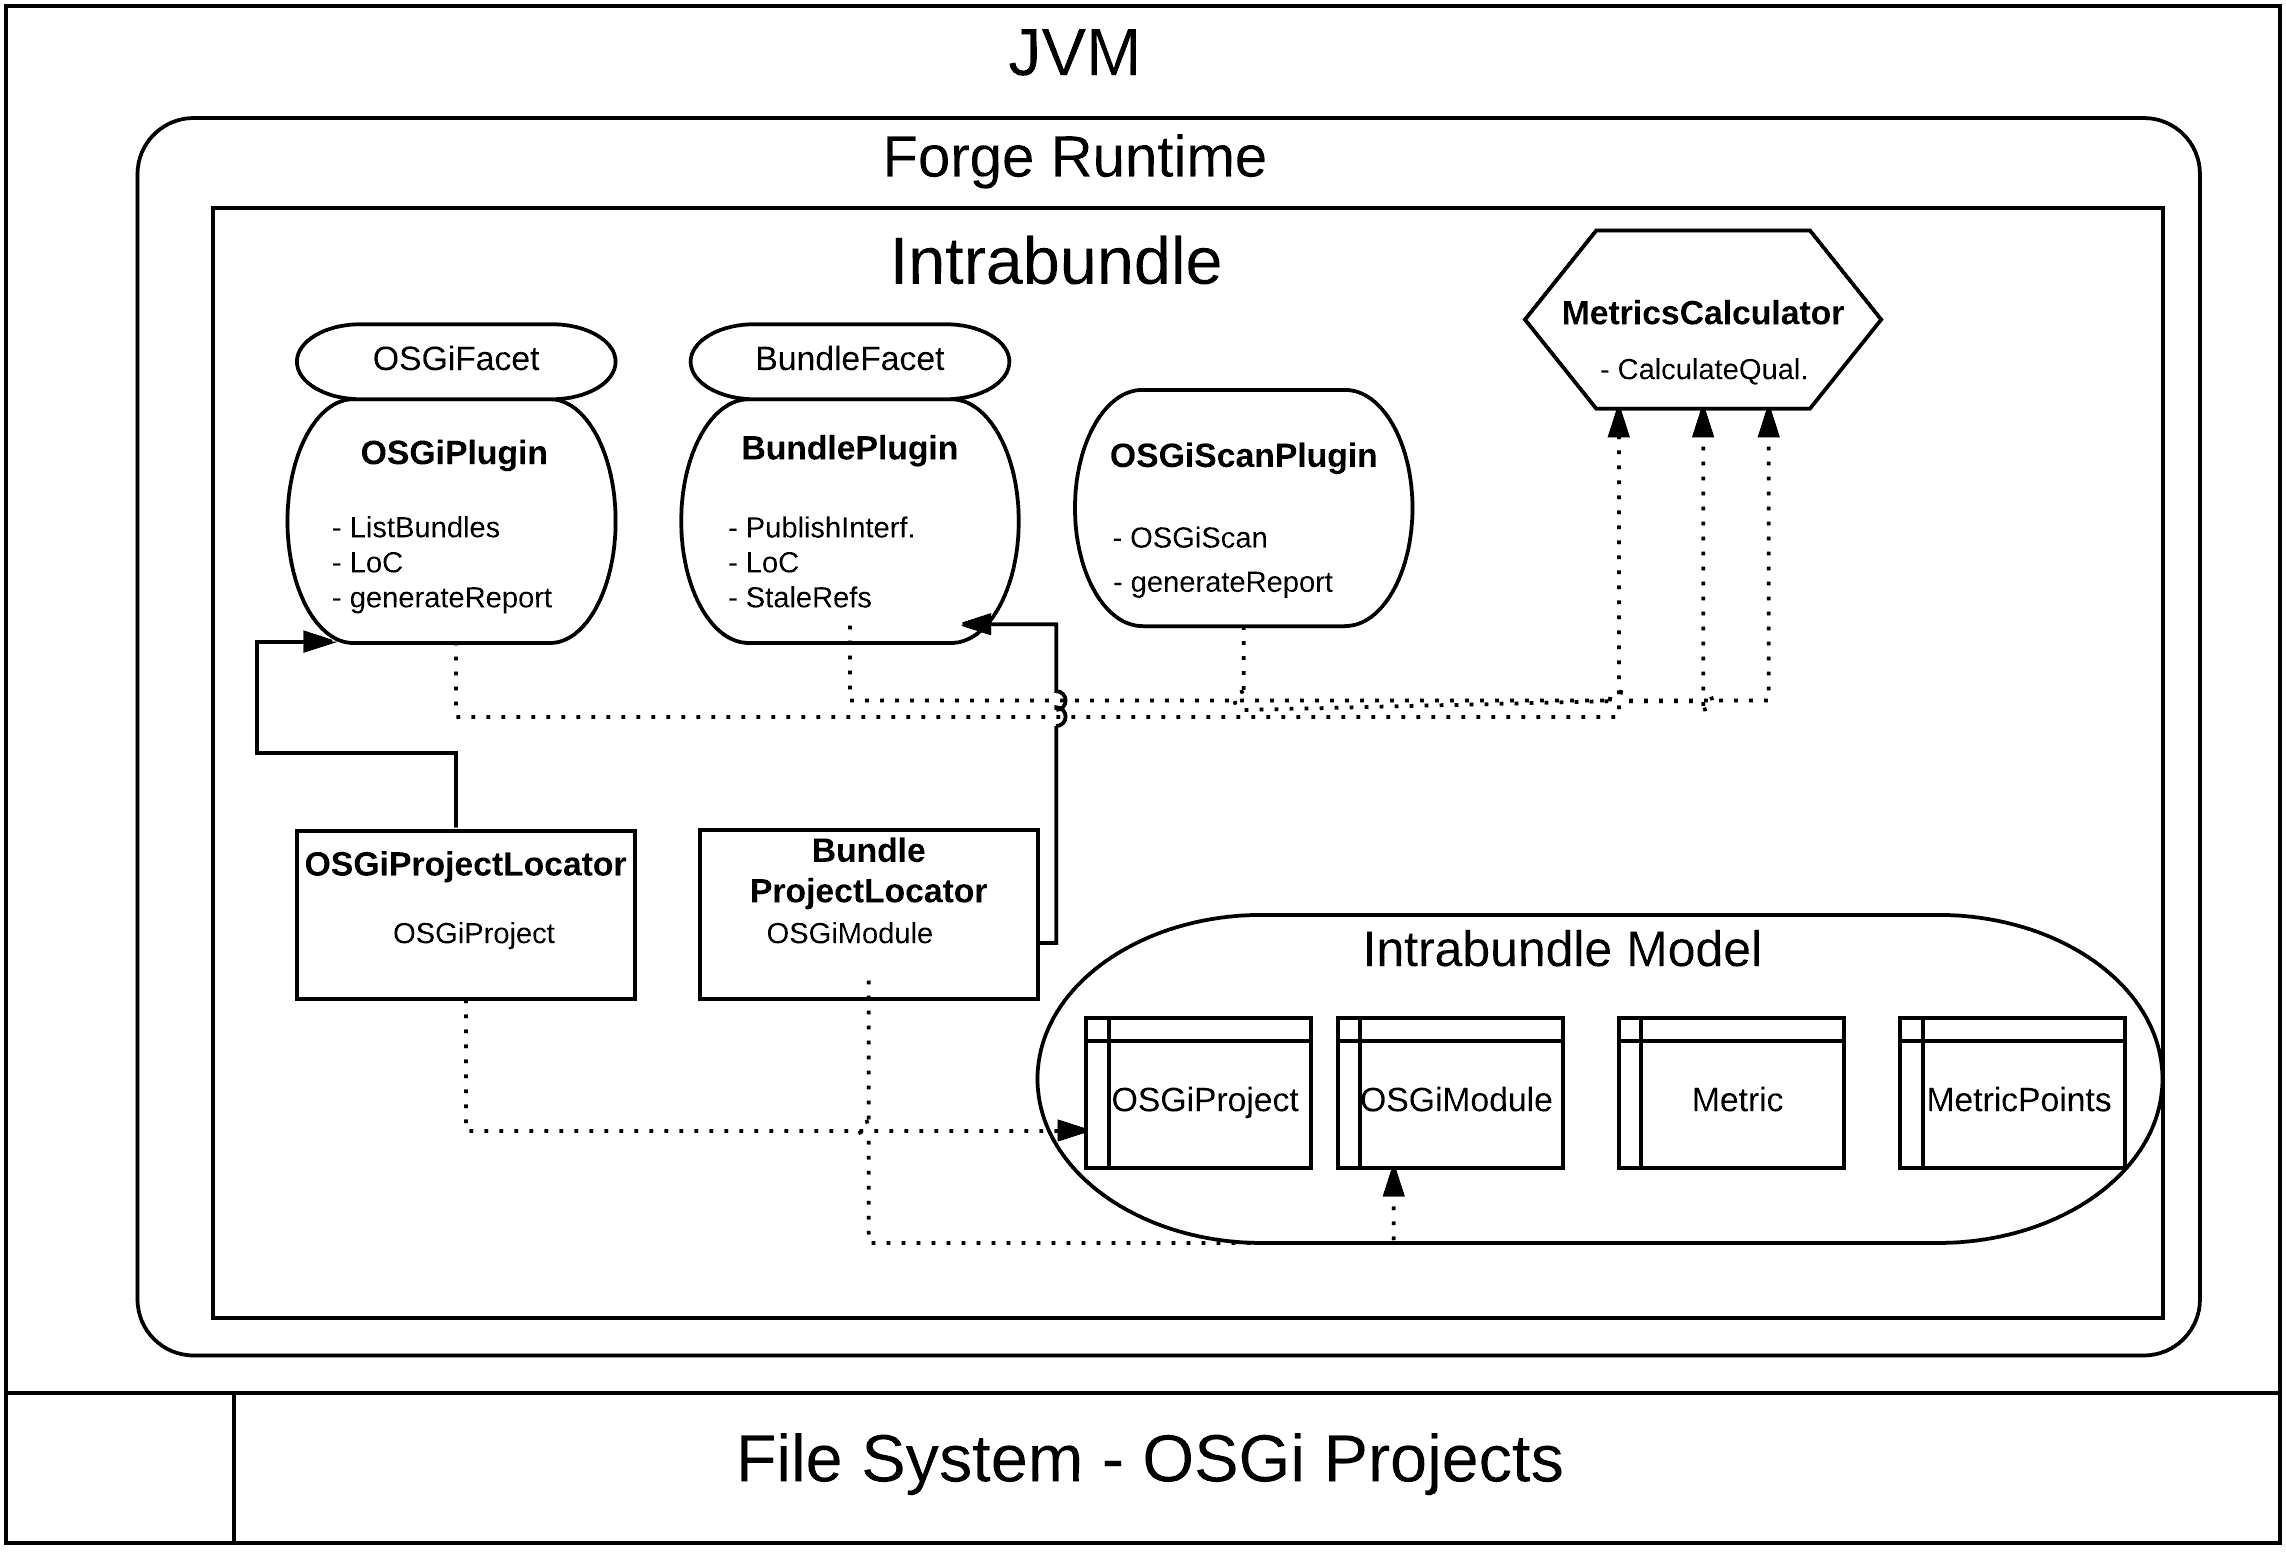
\includegraphics{intrabundle-arch}
\end{figure}  
\FloatBarrier


\section{Identifying OSGi Projects and Bundles}

\section{Collecting Bundle Data}

\section{Metrics Calculation}
The data collected earlier will be materialized into six metrics that will be used to calculate OSGi projects quality  

\section{Intrabundle Quality}
In this section we will see how Intrabundle's quality is managed and how some concepts of \textit{section \ref{sec:quality}} were applied to the project. As the project is not OSGi based we can't apply Intrabundle's metrics on itself so we used classical approaches to assure the quality of the project.

\subsection{Internal quality}
Intrabundle internal is managed by PMD and JaCoCo. PMD is an static analysis tool and JaCoCo a dynamic analysis one. Both were presented at Chapter two in section \textit{Quality Analysis Tools} with the objective to guarantee non functional requirements.

\subsubsection{Example}
 PMD was already illustrated at Chapter 2 as an example of static analysis tool. JaCoCo is used to calculate code coverage to track files and methods that automated tests are covering. Figure 3.1 shows JaCoCo code coverage report for Intrabundle:

\begin{figure}[h]
\caption{Intrabundle code coverage}
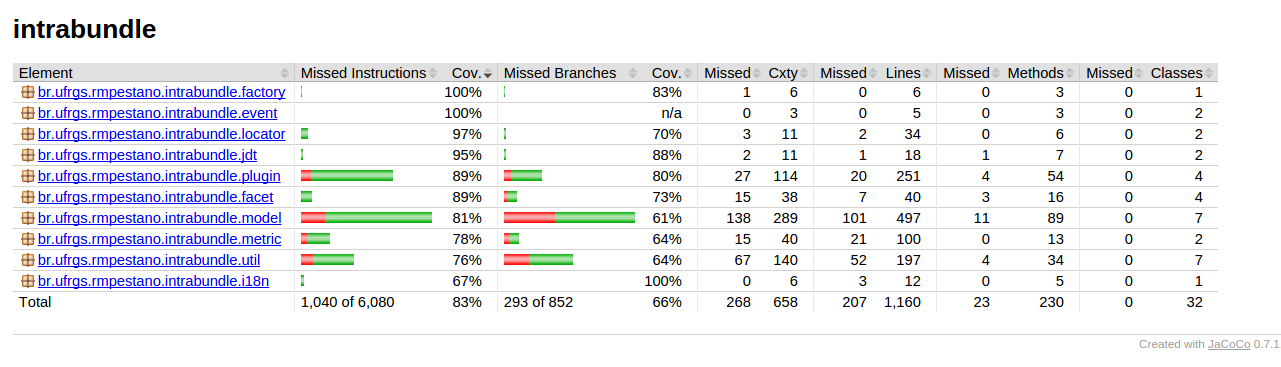
\includegraphics[scale=0.5]{intrabundle-code-coverage}
\end{figure}

\FloatBarrier

\subsection{External quality}
Intrabunde external quality is assured by automated whitebox tests so we can verify if Intrabundle is working as expected, if it meets its functional requirements.

\subsubsection{Example}
As of November 2014 Intrabundle performs 62 \textbf{integration tests} which can be defined as automated tests aimed to detect any inconsistencies between the software units that are integrated together. In this kind of automated tests the system must be running and in case of Intrabundle we also need the Forge runtime up and running during tests and that is done by Arquillian \citep{dan 2011}, an integration test platform. Figure 3.2 shows the result of integration tests execution:

\begin{figure}[h]
\caption{Intrabundle integration tests}
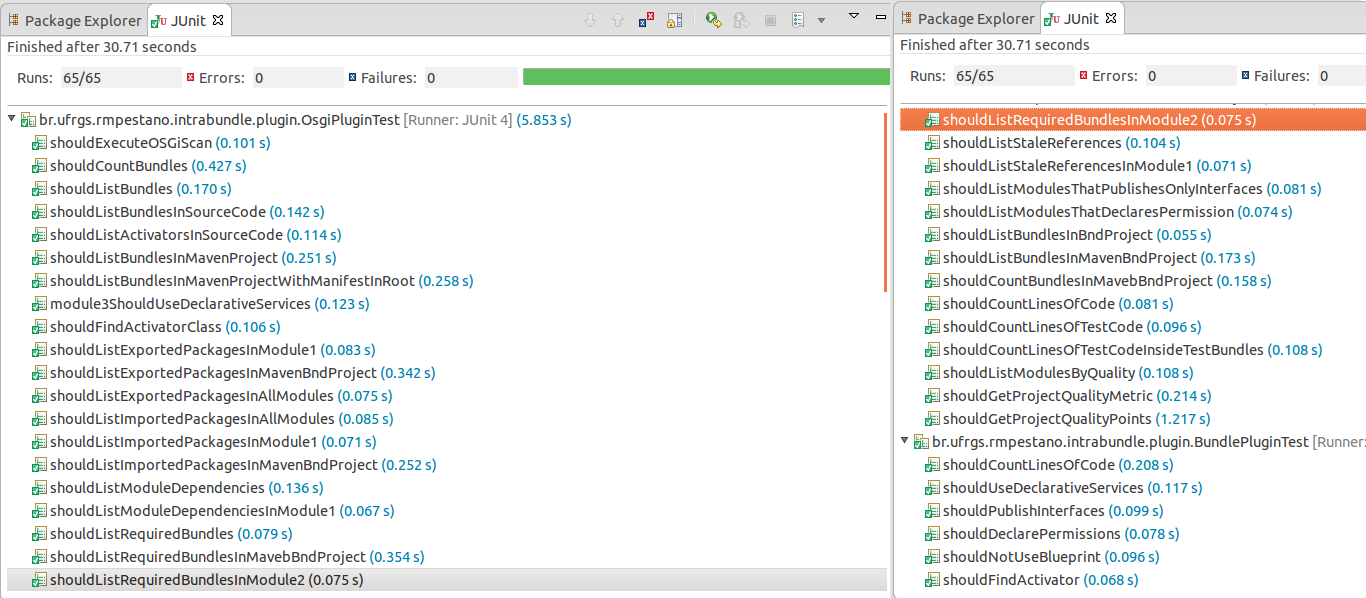
\includegraphics[scale=0.5]{intrabundle-external-quality}
\end{figure}

\FloatBarrier